%%%%%%%%%%%%%%%%%%%%%%%%%%%%%%%%%%%%%%%%%
% Beamer Presentation
% LaTeX Template
% Version 1.0 (10/11/12)
%
% This template has been downloaded from:
% http://www.LaTeXTemplates.com
%
% License:
% CC BY-NC-SA 3.0 (http://creativecommons.org/licenses/by-nc-sa/3.0/)
%
%%%%%%%%%%%%%%%%%%%%%%%%%%%%%%%%%%%%%%%%%

%----------------------------------------------------------------------------------------
%	PACKAGES AND THEMES
%----------------------------------------------------------------------------------------

\documentclass{beamer}

\mode<presentation> {

% The Beamer class comes with a number of default slide themes
% which change the colors and layouts of slides. Below this is a list
% of all the themes, uncomment each in turn to see what they look like.

%\usetheme{default}
%\usetheme{AnnArbor}
%\usetheme{Antibes}
%\usetheme{Bergen}
%\usetheme{Berkeley}
%\usetheme{Berlin}
%\usetheme{Boadilla}
%\usetheme{CambridgeUS}
%\usetheme{Copenhagen}
%\usetheme{Darmstadt}
%\usetheme{Dresden}
%\usetheme{Frankfurt}
%\usetheme{Goettingen}
%\usetheme{Hannover}
%\usetheme{Ilmenau}
%\usetheme{JuanLesPins}
%\usetheme{Luebeck}
\usetheme{Madrid}
%\usetheme{Malmoe}
%\usetheme{Marburg}
%\usetheme{Montpellier}
%\usetheme{PaloAlto}
%\usetheme{Pittsburgh}
%\usetheme{Rochester}
%\usetheme{Singapore}
%\usetheme{Szeged}
%\usetheme{Warsaw}

% As well as themes, the Beamer class has a number of color themes
% for any slide theme. Uncomment each of these in turn to see how it
% changes the colors of your current slide theme.

%\usecolortheme{albatross}
%\usecolortheme{beaver}
%\usecolortheme{beetle}
%\usecolortheme{crane}
%\usecolortheme{dolphin}
%\usecolortheme{dove}
%\usecolortheme{fly}
%\usecolortheme{lily}
%\usecolortheme{orchid}
%\usecolortheme{rose}
%\usecolortheme{seagull}
%\usecolortheme{seahorse}
%\usecolortheme{whale}
%\usecolortheme{wolverine}

%\setbeamertemplate{footline} % To remove the footer line in all slides uncomment this line
%\setbeamertemplate{footline}[page number] % To replace the footer line in all slides with a simple slide count uncomment this line

%\setbeamertemplate{navigation symbols}{} % To remove the navigation symbols from the bottom of all slides uncomment this line
}

\usepackage{graphicx} % Allows including images
\usepackage{booktabs} % Allows the use of \toprule, \midrule and \bottomrule in tables
\usepackage{algorithmic}
\usepackage{tikz}
\usetikzlibrary{calc,arrows.meta,positioning, bending}


%----------------------------------------------------------------------------------------
%	TITLE PAGE
%----------------------------------------------------------------------------------------

\title[Tarski]{Tarski Fixed Point Computation and the Arrival Problem} % The short title appears at the bottom of every slide, the full title is only on the title page

\author{Angus Joshi} % Your name
\institute[UoE] % Your institution as it will appear on the bottom of every slide, may be shorthand to save space
{
University of Edinburgh \\ % Your institution for the title page
\medskip
\textit{s1712180@ed.ac.uk} % Your email address
}
\date{\today} % Date, can be changed to a custom date

\begin{document}

\begin{frame}
\titlepage % Print the title page as the first slide
\end{frame}

\begin{frame}
\frametitle{Overview} % Table of contents slide, comment this block out to remove it
\tableofcontents % Throughout your presentation, if you choose to use \section{} and \subsection{} commands, these will automatically be printed on this slide as an overview of your presentation
\end{frame}

%----------------------------------------------------------------------------------------
%	PRESENTATION SLIDES
%----------------------------------------------------------------------------------------

%------------------------------------------------
\section{Basic Definitions and Algorithmic Results} % Sections can be created in order to organize your presentation into discrete blocks, all sections and subsections are automatically printed in the table of contents as an overview of the talk
%------------------------------------------------

\subsection{The integer lattice, monotone functions, Tarski's theorem} % A subsection can be created just before a set of slides with a common theme to further break down your presentation into chunks

\begin{frame}
\frametitle{The integer lattice, monotone functions, Tarski's theorem}
    \begin{definition}[Bounded Integer Lattice]
        The \emph{bounded d-dimensional integer lattice} $[N]^d = \{1, ..., N\}^d$ is equipped with a lattice ordering
        where for $(x_1, ..., x_d), (x_1', ..., x'_d) \in [N]^d$, $(x_1, ..., x_d) \leq (x_1', ..., x'_d)$ if
        $x_i \leq x'_i$ for each $i \in [d]$.
    \end{definition}
    \begin{definition}[Monotone function] 
        A function $f : [N]^d \to [N]^d$ is monotone if whenever $x, x' \in [N]^d$ with $x \leq x'$, $f(x) \leq f(x')$.
    \end{definition}
    \begin{Theorem}[Tarski]
        If $f : [N]^d \to [N]^d$ is monotone, then there is a point $x \in [N]^d$ with $f(x) = x$.
    \end{Theorem}
\end{frame}

\subsection{The problem, Lower bounds}
%------------------------------------------------

\begin{frame}
\frametitle{The problem, Lower Bounds}
    \begin{Definition}[\textsc{Tarski}]
        The problem $\textsc{Tarski}(N, d)$ is, given oracle access to a monotone function $f : [N]^d \to [N]^d$, find a point $x \in [N]^d$ such that
        $f(x) = x$.
    \end{Definition}
    \begin{Theorem}[Etessami, Papadimitriou, Rubinstein, Yannakakis]
        The query complexity of $\textsc{Tarski}(N, 2)$ is $\Theta(\log^2 N)$.
    \end{Theorem}
    \begin{Corollary}
        The query complexity of $\textsc{Tarski}(N, d)$ is $\Omega(\log^2 N)$ for $d \geq 2$.
    \end{Corollary}
\end{frame}

%------------------------------------------------

\newcommand{\trsk}{\textsc{Tarski }}

\subsection{Known Upper Bounds}
\begin{frame}
\frametitle{Known Upper Bounds}

\begin{Theorem}[Fearnley, Pálvölgyi, Savani]
    The query complexity of $\trsk(N, 3)$ is $\Theta(\log^2 N)$.
\end{Theorem}
\begin{Theorem}[Chen, Li]
    The query complexity of $\trsk(N, d)$ is $O(\log^{\lceil (d+1) / 2 \rceil} N)$.
\end{Theorem}

\end{frame}

%------------------------------------------------

\section{The Arrival Problem}
\subsection{Definitions}
\begin{frame}
\frametitle{The Arrival Problem}
  \begin{figure}[h]
    \centering
    \tikzset{every picture/.style={line width=0.75pt}} %set default line width to 0.75pt        

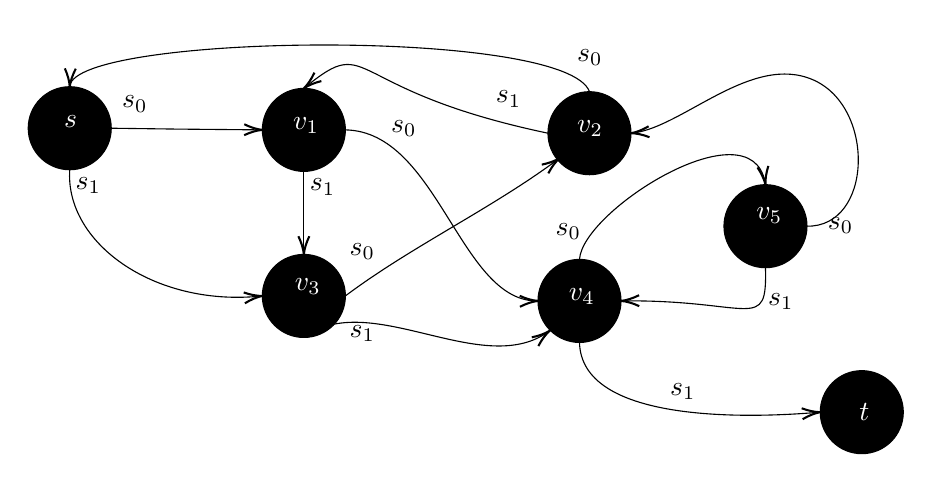
\begin{tikzpicture}[x=0.6pt,y=0.6pt,yscale=-1,xscale=1]
%uncomment if require: \path (0,300); %set diagram left start at 0, and has height of 300

%Shape: Circle [id:dp5495329281078569] 
\draw  [fill={rgb, 255:red, 0; green, 0; blue, 0 }  ,fill opacity=1 ] (32,49) .. controls (32,35.19) and (43.19,24) .. (57,24) .. controls (70.81,24) and (82,35.19) .. (82,49) .. controls (82,62.81) and (70.81,74) .. (57,74) .. controls (43.19,74) and (32,62.81) .. (32,49) -- cycle ;
%Straight Lines [id:da33331850965746734] 
\draw    (82,49) -- (121.98,49.53) -- (171,49.98) ;
\draw [shift={(173,50)}, rotate = 180.52] [color={rgb, 255:red, 0; green, 0; blue, 0 }  ][line width=0.75]    (10.93,-3.29) .. controls (6.95,-1.4) and (3.31,-0.3) .. (0,0) .. controls (3.31,0.3) and (6.95,1.4) .. (10.93,3.29)   ;
%Shape: Circle [id:dp8549825383964691] 
\draw  [fill={rgb, 255:red, 0; green, 0; blue, 0 }  ,fill opacity=1 ] (173,50) .. controls (173,36.19) and (184.19,25) .. (198,25) .. controls (211.81,25) and (223,36.19) .. (223,50) .. controls (223,63.81) and (211.81,75) .. (198,75) .. controls (184.19,75) and (173,63.81) .. (173,50) -- cycle ;
%Straight Lines [id:da15070581279870932] 
\draw    (198,75) -- (198,123) ;
\draw [shift={(198,125)}, rotate = 270] [color={rgb, 255:red, 0; green, 0; blue, 0 }  ][line width=0.75]    (10.93,-3.29) .. controls (6.95,-1.4) and (3.31,-0.3) .. (0,0) .. controls (3.31,0.3) and (6.95,1.4) .. (10.93,3.29)   ;
%Shape: Circle [id:dp4390825091110777] 
\draw  [fill={rgb, 255:red, 0; green, 0; blue, 0 }  ,fill opacity=1 ] (345,52) .. controls (345,38.19) and (356.19,27) .. (370,27) .. controls (383.81,27) and (395,38.19) .. (395,52) .. controls (395,65.81) and (383.81,77) .. (370,77) .. controls (356.19,77) and (345,65.81) .. (345,52) -- cycle ;
%Shape: Circle [id:dp9757305512769809] 
\draw  [fill={rgb, 255:red, 0; green, 0; blue, 0 }  ,fill opacity=1 ] (173,150) .. controls (173,136.19) and (184.19,125) .. (198,125) .. controls (211.81,125) and (223,136.19) .. (223,150) .. controls (223,163.81) and (211.81,175) .. (198,175) .. controls (184.19,175) and (173,163.81) .. (173,150) -- cycle ;
%Shape: Circle [id:dp6476109813645592] 
\draw  [fill={rgb, 255:red, 0; green, 0; blue, 0 }  ,fill opacity=1 ] (339,153) .. controls (339,139.19) and (350.19,128) .. (364,128) .. controls (377.81,128) and (389,139.19) .. (389,153) .. controls (389,166.81) and (377.81,178) .. (364,178) .. controls (350.19,178) and (339,166.81) .. (339,153) -- cycle ;
%Shape: Circle [id:dp9387189635111892] 
\draw  [fill={rgb, 255:red, 0; green, 0; blue, 0 }  ,fill opacity=1 ] (451,108) .. controls (451,94.19) and (462.19,83) .. (476,83) .. controls (489.81,83) and (501,94.19) .. (501,108) .. controls (501,121.81) and (489.81,133) .. (476,133) .. controls (462.19,133) and (451,121.81) .. (451,108) -- cycle ;
%Shape: Circle [id:dp6728900489022538] 
\draw  [fill={rgb, 255:red, 0; green, 0; blue, 0 }  ,fill opacity=1 ] (509,220) .. controls (509,206.19) and (520.19,195) .. (534,195) .. controls (547.81,195) and (559,206.19) .. (559,220) .. controls (559,233.81) and (547.81,245) .. (534,245) .. controls (520.19,245) and (509,233.81) .. (509,220) -- cycle ;
%Curve Lines [id:da06839655673782064] 
\draw    (223,50) .. controls (278.44,50.99) and (291.74,151.95) .. (337.6,153) ;
\draw [shift={(339,153)}, rotate = 178.78] [color={rgb, 255:red, 0; green, 0; blue, 0 }  ][line width=0.75]    (10.93,-3.29) .. controls (6.95,-1.4) and (3.31,-0.3) .. (0,0) .. controls (3.31,0.3) and (6.95,1.4) .. (10.93,3.29)   ;
%Curve Lines [id:da30024168681774177] 
\draw    (364,178) .. controls (364.99,225.52) and (461.05,224.04) .. (507.6,220.12) ;
\draw [shift={(509,220)}, rotate = 175.03] [color={rgb, 255:red, 0; green, 0; blue, 0 }  ][line width=0.75]    (10.93,-3.29) .. controls (6.95,-1.4) and (3.31,-0.3) .. (0,0) .. controls (3.31,0.3) and (6.95,1.4) .. (10.93,3.29)   ;
%Curve Lines [id:da031177664907863667] 
\draw    (370,27) .. controls (356.28,-11.22) and (69.81,-8.14) .. (57.41,22.11) ;
\draw [shift={(57,24)}, rotate = 271.79] [color={rgb, 255:red, 0; green, 0; blue, 0 }  ][line width=0.75]    (10.93,-3.29) .. controls (6.95,-1.4) and (3.31,-0.3) .. (0,0) .. controls (3.31,0.3) and (6.95,1.4) .. (10.93,3.29)   ;
%Curve Lines [id:da19551484489395188] 
\draw    (364,128) .. controls (365.79,98.44) and (466.95,34.79) .. (475.76,81.55) ;
\draw [shift={(476,83)}, rotate = 261.95] [color={rgb, 255:red, 0; green, 0; blue, 0 }  ][line width=0.75]    (10.93,-3.29) .. controls (6.95,-1.4) and (3.31,-0.3) .. (0,0) .. controls (3.31,0.3) and (6.95,1.4) .. (10.93,3.29)   ;
%Curve Lines [id:da5453571551089418] 
\draw    (345,52) .. controls (220.26,25.76) and (239.59,-8.8) .. (199.24,23.99) ;
\draw [shift={(198,25)}, rotate = 320.6] [color={rgb, 255:red, 0; green, 0; blue, 0 }  ][line width=0.75]    (10.93,-3.29) .. controls (6.95,-1.4) and (3.31,-0.3) .. (0,0) .. controls (3.31,0.3) and (6.95,1.4) .. (10.93,3.29)   ;
%Curve Lines [id:da7736997926226343] 
\draw    (223,150) .. controls (262.6,120.3) and (311.02,97.46) .. (350.8,67.9) ;
\draw [shift={(352,67)}, rotate = 143.13] [color={rgb, 255:red, 0; green, 0; blue, 0 }  ][line width=0.75]    (10.93,-3.29) .. controls (6.95,-1.4) and (3.31,-0.3) .. (0,0) .. controls (3.31,0.3) and (6.95,1.4) .. (10.93,3.29)   ;
%Curve Lines [id:da35489757719958615] 
\draw    (57,74) .. controls (54.03,117.56) and (106.93,156.22) .. (171.05,150.2) ;
\draw [shift={(173,150)}, rotate = 173.85] [color={rgb, 255:red, 0; green, 0; blue, 0 }  ][line width=0.75]    (10.93,-3.29) .. controls (6.95,-1.4) and (3.31,-0.3) .. (0,0) .. controls (3.31,0.3) and (6.95,1.4) .. (10.93,3.29)   ;
%Curve Lines [id:da7424500525745132] 
\draw    (198,175) .. controls (237.6,145.3) and (304.64,199.89) .. (344.79,171.87) ;
\draw [shift={(346,171)}, rotate = 143.13] [color={rgb, 255:red, 0; green, 0; blue, 0 }  ][line width=0.75]    (10.93,-3.29) .. controls (6.95,-1.4) and (3.31,-0.3) .. (0,0) .. controls (3.31,0.3) and (6.95,1.4) .. (10.93,3.29)   ;
%Curve Lines [id:da3132040250840804] 
\draw    (501,108) .. controls (540.44,108.6) and (542.5,36.73) .. (505,20) .. controls (468.25,3.6) and (426.87,47.76) .. (396.83,51.8) ;
\draw [shift={(395,52)}, rotate = 355.43] [color={rgb, 255:red, 0; green, 0; blue, 0 }  ][line width=0.75]    (10.93,-3.29) .. controls (6.95,-1.4) and (3.31,-0.3) .. (0,0) .. controls (3.31,0.3) and (6.95,1.4) .. (10.93,3.29)   ;
%Curve Lines [id:da9721751571878057] 
\draw    (476,133) .. controls (477,172.8) and (468.09,152.21) .. (390.18,152.99) ;
\draw [shift={(389,153)}, rotate = 359.27] [color={rgb, 255:red, 0; green, 0; blue, 0 }  ][line width=0.75]    (10.93,-3.29) .. controls (6.95,-1.4) and (3.31,-0.3) .. (0,0) .. controls (3.31,0.3) and (6.95,1.4) .. (10.93,3.29)   ;

% Text Node
\draw (87,28) node [anchor=north west][inner sep=0.75pt]   [align=left] {$\displaystyle s_{0}$};
% Text Node
\draw (52,40) node [anchor=north west][inner sep=0.75pt]  [color={rgb, 255:red, 255; green, 255; blue, 255 }  ,opacity=1 ] [align=left] {$\displaystyle s$};
% Text Node
\draw (59,77) node [anchor=north west][inner sep=0.75pt]   [align=left] {$\displaystyle s_{1}$};
% Text Node
\draw (249,43) node [anchor=north west][inner sep=0.75pt]   [align=left] {$\displaystyle s_{0}$};
% Text Node
\draw (190,41) node [anchor=north west][inner sep=0.75pt]  [color={rgb, 255:red, 255; green, 255; blue, 255 }  ,opacity=1 ] [align=left] {$\displaystyle v_{1}$};
% Text Node
\draw (200,78) node [anchor=north west][inner sep=0.75pt]   [align=left] {$\displaystyle s_{1}$};
% Text Node
\draw (361,0) node [anchor=north west][inner sep=0.75pt]   [align=left] {$\displaystyle s_{0}$};
% Text Node
\draw (361,43) node [anchor=north west][inner sep=0.75pt]  [color={rgb, 255:red, 255; green, 255; blue, 255 }  ,opacity=1 ] [align=left] {$\displaystyle v_{2}$};
% Text Node
\draw (224,117) node [anchor=north west][inner sep=0.75pt]   [align=left] {$\displaystyle s_{0}$};
% Text Node
\draw (191,138) node [anchor=north west][inner sep=0.75pt]  [color={rgb, 255:red, 255; green, 255; blue, 255 }  ,opacity=1 ] [align=left] {$\displaystyle v_{3}$};
% Text Node
\draw (224,166) node [anchor=north west][inner sep=0.75pt]   [align=left] {$\displaystyle s_{1}$};
% Text Node
\draw (348,105) node [anchor=north west][inner sep=0.75pt]   [align=left] {$\displaystyle s_{0}$};
% Text Node
\draw (356,144) node [anchor=north west][inner sep=0.75pt]  [color={rgb, 255:red, 255; green, 255; blue, 255 }  ,opacity=1 ] [align=left] {$\displaystyle v_{4}$};
% Text Node
\draw (417,201) node [anchor=north west][inner sep=0.75pt]   [align=left] {$\displaystyle s_{1}$};
% Text Node
\draw (512,101) node [anchor=north west][inner sep=0.75pt]   [align=left] {$\displaystyle s_{0}$};
% Text Node
\draw (469,95) node [anchor=north west][inner sep=0.75pt]  [color={rgb, 255:red, 255; green, 255; blue, 255 }  ,opacity=1 ] [align=left] {$\displaystyle v_{5}$};
% Text Node
\draw (476,147) node [anchor=north west][inner sep=0.75pt]   [align=left] {$\displaystyle s_{1}$};
% Text Node
\draw (531,213) node [anchor=north west][inner sep=0.75pt]  [color={rgb, 255:red, 255; green, 255; blue, 255 }  ,opacity=1 ] [align=left] {$\displaystyle t$};
% Text Node
\draw (312,25) node [anchor=north west][inner sep=0.75pt]   [align=left] {$\displaystyle s_{1}$};


\end{tikzpicture}

  \end{figure}
\end{frame}

\begin{frame}
\begin{figure}[ht]
  \frametitle{Finiteness}
  \centering
  \tikzset{every picture/.style={line width=0.75pt}} %set default line width to 0.75pt        
  \raisebox{-0.62\height}{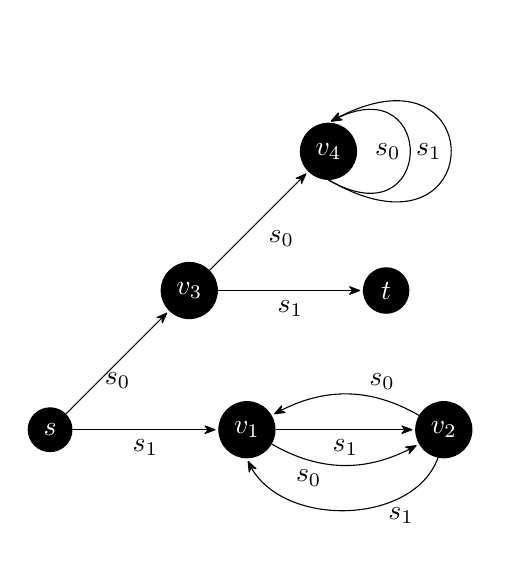
\begin{tikzpicture}[x=0.6pt,y=0.6pt,yscale=-1,xscale=1, 
  main/.style = {draw, circle, 
  fill={rgb, 255:red, 0; green, 0; blue, 0 }},
  text=white,
  node distance=2.5cm,
  ->,
  >={Stealth[round,sep]}]
  \node[main] (s) {$s$};
  \node[main] (1) [right of=s]{$v_1$};
  \node[main] (2) [right of=1]{$v_2$};
  \node[main] (3) [above right of=s]{$v_3$};
  \node[main] (4) [above right of=3]{$v_4$};
  
  % \node[main] (4) [right of=3]{$v_n$};
  \node[main] (t)[right of=3]{$t$};
  \draw (s) -- (3) node[midway, below, text=black]{$s_0$};
  \draw (s) -- (1) node[midway, below, text=black]{$s_1$};
  \draw (1) -- (2) node[midway, below, text=black]{$s_1$};
  \draw (3) -- (t) node[midway, below, text=black]{$s_1$};
  \draw (3) -- (4) node[midway, below right, text=black]{$s_0$};
  \draw (2) edge[bend left] node[near start, above, text=black]{$s_0$} (1);
  \draw (1) edge[bend left] node[near start, below, text=black]{$s_0$}(2);

  \draw (4.south) to[bend left=120, min distance=1.6cm] node[midway, left, text=black]{$s_0$} (4.north);
  \draw (4.south) to[bend left=120, min distance=2.4cm] node[midway, left, text=black]{$s_1$} (4.north);
  % \draw (4) edge[bend left] node[near start, above, text=black]{$s_0$}(1);
  \draw (2) edge[bend right=70, min distance=0.8cm] node[near start, below, text=black]{$s_1$} (1.south);
\end{tikzpicture}
}
  \hfil
  $\mapsto$
  \hfil
  \raisebox{-0.5\height}{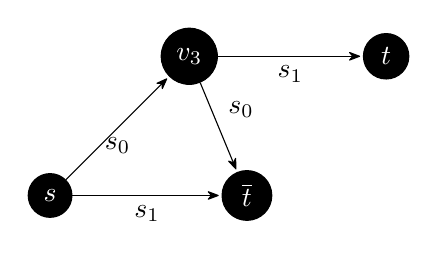
\begin{tikzpicture}[x=0.6pt,y=0.6pt,yscale=-1,xscale=1, 
  main/.style = {draw, circle, 
  fill={rgb, 255:red, 0; green, 0; blue, 0 }},
  text=white,
  node distance=2.5cm,
  ->,
  >={Stealth[round,sep]}]
  \node[main] (s) {$s$};
  \node[main] (1) [right of=s]{$\overline{t}$};
  \node[main] (3) [above right of=s]{$v_3$};
  
  % \node[main] (4) [right of=3]{$v_n$};
  \node[main] (4)[right of=3]{$t$};
  \draw (s) -- (3) node[midway, below, text=black]{$s_0$};
  \draw (s) -- (1) node[midway, below, text=black]{$s_1$};
  \draw (3) -- (4) node[midway, below, text=black]{$s_1$};
  \draw (3) -- (1) node[midway, above right, text=black]{$s_0$};
\end{tikzpicture}
}
  \end{figure}
  \end{frame}

\begin{frame}
\frametitle{Long Walks}
  \begin{figure}[h]
    \centering
    \tikzset{every picture/.style={line width=0.75pt}} %set default line width to 0.75pt        

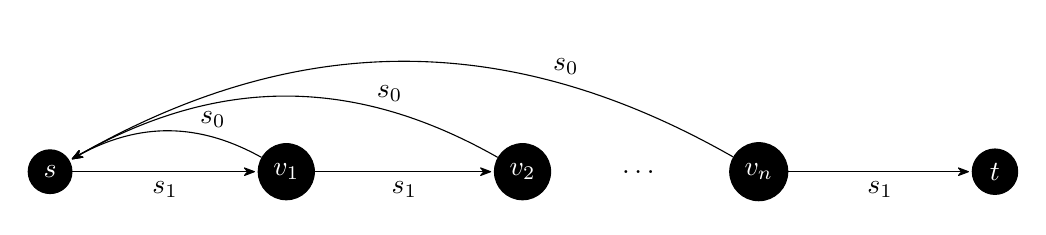
\begin{tikzpicture}[x=0.6pt,y=0.6pt,yscale=-1,xscale=1, 
  main/.style = {draw, circle, 
  fill={rgb, 255:red, 0; green, 0; blue, 0 }},
  text=white,
  node distance=3cm,
  ->,
  >={Stealth[round,sep]}]
  \node[main] (1) {$s$};
  \node[main] (2) [right of=1]{$v_1$};
  \node[main] (3) [right of=2]{$v_2$};
  \node[main] (4) [right of=3]{$v_n$};
  \node[main] (5)[right of=4]{$t$};
  \node[text=black] at ($(3)!.5!(4)$) {\ldots};
  \draw (1) -- (2) node[midway, below, text=black]{$s_1$};
  \draw (2) -- (3) node[midway, below, text=black]{$s_1$};
  \draw (4) -- (5) node[midway, below, text=black]{$s_1$};
  % \path (1) edge[loop above] node {$s_0$} (1);
  \draw (2) edge[bend left] node[near start, above, text=black]{$s_0$} (1);
  \draw (3) edge[bend left] node[near start, above, text=black]{$s_0$}(1);
  \draw (4) edge[bend left] node[near start, above, text=black]{$s_0$}(1);
\end{tikzpicture}

  \end{figure}
\end{frame}


\subsection{Reduction to \textsc{Tarski}}
\begin{frame}
\frametitle{Reduction to \textsc{Tarski}}
    \begin{Theorem}[Gärtner, Haslebacher, Hoang]
        \textsc{Arrival} is polynomial-time reducible to \textsc{Tarski}.
    \end{Theorem}
\end{frame}

%------------------------------------------------

\section{Progress, Next Steps, Open Questions}
\subsection{Testing the Algorithms}
\begin{frame}
\frametitle{Testing the Algorithms}
    \begin{figure}[t]
        \centering
        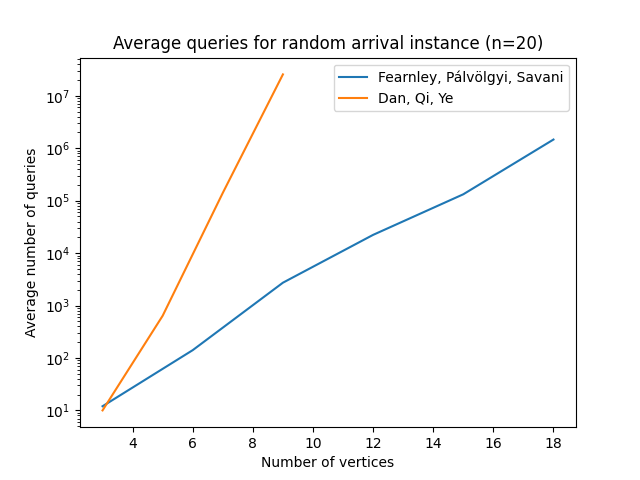
\includegraphics[width=2.2in]{avQueries.png}
        \centering
        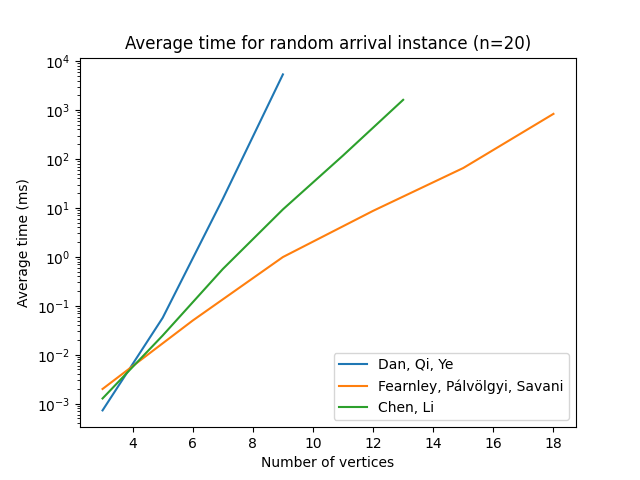
\includegraphics[width=2.2in]{avTime.png}
    \end{figure}
\end{frame}

\begin{frame}
\frametitle{Reality}
    \begin{figure}[t]
        \centering
        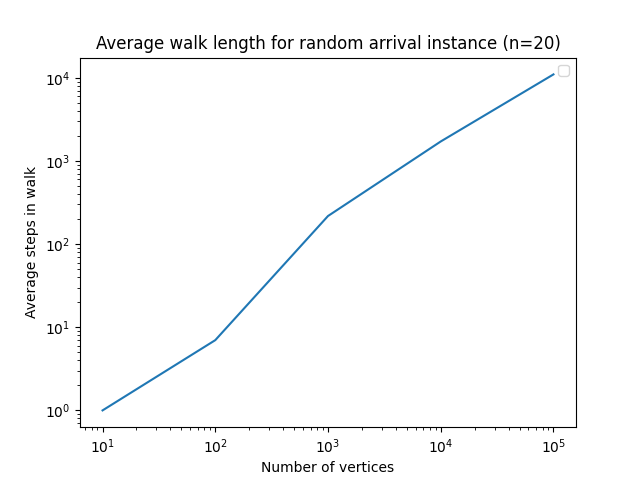
\includegraphics[width=2.2in]{walkLength.png}
        \centering
        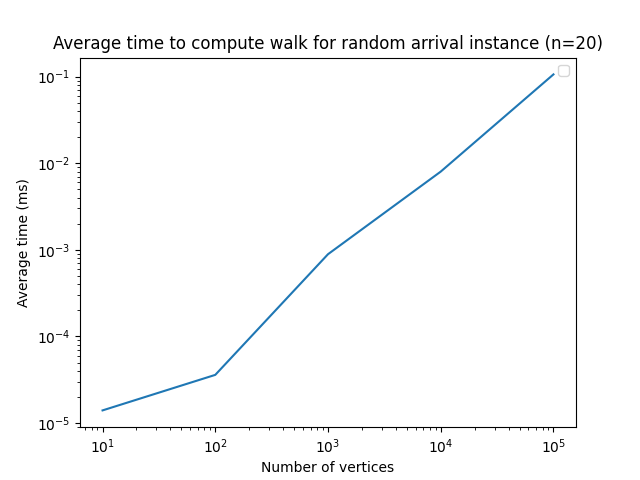
\includegraphics[width=2.2in]{walkTime.png}
    \end{figure}
    
\end{frame}

\subsection{Progress, Next Steps, Open Problems}
\newcommand{\pav}{Pálvölgyi}
\begin{frame}
\frametitle{Progress and Next Steps}
    \begin{itemize}
        \item Progress
        \begin{itemize}
            \item Explored solving the 4-dimensional \trsk problem,
            \item Implemented Fearnley, \pav, Savani algorithm,
            \item Applied the algorithm to randomly generated instances of \textsc{Arrival}.
        \end{itemize}
        \item Next Steps
        \begin{itemize}
            \item Explore solving the 4-dimensional \trsk problem in the special case of monotone functions
            corresponding to arrival instances.
        \end{itemize}
      \item Open Problems
        \begin{itemize}
          \item Is \textsc{Tarski} fixed-parameter tractable? That is, is the query complexity of $\textsc{Tarski}(N, d)$ $\Theta(\log^2n)$ for fixed $d$?
          \item Is \textsc{Tarski} fixed-parameter tractable in the special case of monotone functions from \textsc{Arrival}?
        \end{itemize}
    \end{itemize}
\end{frame}

\end{document}
